%!TEX TS-program = xelatex

\documentclass[xcolor=table, t]{beamer}

\usetheme{Hannover}
\usecolortheme{rose}

%%% Работа с русским языком
\usepackage[english,russian]{babel}   %% загружает пакет многоязыковой вёрстки
\usepackage{fontspec,xltxtra,xunicode}      %% подготавливает загрузку шрифтов Open Type, True Type и др.
%\defaultfontfeatures{Ligatures={TeX},Renderer=Basic}  %% свойства шрифтов по умолчанию
\setmainfont[Ligatures={TeX,Historic},
SmallCapsFont={Brill},
SmallCapsFeatures={Letters=SmallCaps}]{Brill} %% задаёт основной шрифт документа
\setsansfont{Brill}                    %% задаёт шрифт без засечек
\setmonofont[Ligatures=NoCommon]{Droid Sans Fallback}
\newfontfamily\JAP{Droid Sans Fallback}
\newfontfamily\ABY{Abyssinica SIL}
\newfontfamily\HEB{Arial}
\newfontfamily\MON{Andale Mono}
\newfontfamily\NAST{Noto Nastaliq Urdu}
\newfontfamily\NASKH{Noto Naskh Arabic}
%\usepackage{indentfirst}
%%% Дополнительная работа с математикой
\usepackage{amsmath,amsfonts,amssymb,amsthm,mathtools} % AMS
\usepackage{icomma} % "Умная" запятая: $0,2$ --- число, $0, 2$ --- перечисление

%%% Работа с картинками
\usepackage{wrapfig} % Обтекание рисунков текстом
\usepackage{rotating}
\usepackage{fixltx2e}
\usepackage{hhline}
\usepackage{lscape}

%%% Работа с таблицами
\usepackage{array,tabularx,tabulary,booktabs} % Дополнительная работа с таблицами
\usepackage{longtable}  % Длинные таблицы
\usepackage{multirow} % Слияние строк в таблице

\usepackage{multicol} % Несколько колонок
%%% Страница
%\usepackage{fancyhdr} % Колонтитулы
% 	\pagestyle{fancy}
 	%\renewcommand{\headrulewidth}{0pt}  % Толщина линейки, отчеркивающей верхний колонтитул
% 	\lfoot{Нижний левый}
% 	\rfoot{Нижний правый}
% 	\rhead{Верхний правый}
% 	\chead{Верхний в центре}
% 	\lhead{Верхний левый}
%	\cfoot{Нижний в центре} % По умолчанию здесь номер страницы

\usepackage{setspace} % Интерлиньяж
%\onehalfspacing % Интерлиньяж 1.5
%\doublespacing % Интерлиньяж 2
\singlespacing % Интерлиньяж 1

\usepackage{subfig} % подкартинки
\usepackage{lastpage} % Узнать, сколько всего страниц в документе.
\usepackage{soul} % Модификаторы начертания
\usepackage{bbding}
\usepackage{tikz} % Работа с графикой
\usepackage{pgfplots}
\usepackage{pgfplotstable}
\usepackage{verbatim}

\usepackage{attachfile2}
\usepackage{alltt}

%%% Лингвистические пакеты
%\usepackage{savetrees} % пакет, который экономит место
\usepackage{forest} % для рисования деревьев
\usepackage{vowel} % для рисования трапеций гласных
\usepackage{natbib}
\bibpunct[: ]{[}{]}{;}{a}{}{,}
\usepackage[nogroupskip,nopostdot, nonumberlist]{glossaries}
%\usepackage{glossary-mcols} 
%\setglossarystyle{mcolindex}
\usepackage{philex} % пакет для примеров
\newcommand{\mytem}{\item[$\circ$]}
\addto\captionsrussian{
\renewcommand{\refname}{}}

\usetikzlibrary{patterns}

\usepackage{ulem}
\usepackage[absolute,overlay]{textpos}
\usepackage{hyperref}
\hypersetup{ % Гиперссылки
	colorlinks=true, % false: ссылки в рамках; true: цветные ссылки
	linkcolor=black, % внутренние ссылки
	citecolor=black, % на библиографию
	filecolor=black, % на файлы
	urlcolor=blue % на URL
	}
\setbeamercolor{alerted text}{fg=blue}
\setbeamerfont{frametitle}{size=\large}
%\setbeamersize{text margin left=4mm,text margin right=1mm} 
\setlength{\parindent}{0em}
\setbeamertemplate{frametitle}[default][center]
\addtobeamertemplate{frametitle}{\vspace*{-0.1mm}}{\vspace*{-0.3cm}}
%\addtobeamertemplate{frametitle}{\vspace{-0.5\baselineskip}}
\setbeamertemplate{navigation symbols}{
	\usebeamerfont{footline}%
    \usebeamercolor[fg]{footline}%
    %\hspace{1em}%
    {{\tiny презентация доступна: \href{tinyurl.com/y3cvqyyr}{\textbf{tinyurl.com/y3cvqyyr}}}
    \hspace{6.7cm}
    \insertframenumber/\inserttotalframenumber\vspace{0.5mm}}}
% начало
\title[]{Письменности мира}
\subtitle{типология, развитие и компоненты}
\author[]{Г. Мороз}
\date{4 октября 2019}
\begin{document}
\frame{\titlepage}
\begin{frame}{План}
\begin{itemize}
\item от меня кто-то возможно ожидал:
\begin{center}
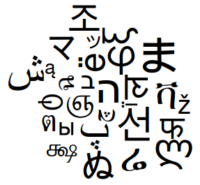
\includegraphics[width=0.3\linewidth]{scripts.png}
\end{center}
\item сегодня я расскажу о
\begin{itemize}
\item разных классификациях систем письма
\item параметрах, необходимые для описания графического знака
\item том, как происходит развитие систем письма вообще
\item том, как происходило развитие систем письма на Земле
\item соотношении письма и языка
\item о компонентах систем письма
\end{itemize}
\end{itemize}
\vfill
Потренироваться в угадывании разных систем письма \href{https://goo.gl/forms/Bue8K65PxTLgeJlZ2}{предлагаю самостоятельно}.
\end{frame}
\section{типология}
\subsection{\citep{taylor83}}
\begin{frame}{Типология систем письма: \citep{taylor83}}
Исаак Тейлор предложил эволюционную модель систем письма:
\begin{itemize}
\item рисунки
\item пиктографическое письмо
\item идеограмматическое письмо
\item силлабическое письмо
\item алфавитное письмо
\end{itemize}
Первые три этапа считались идиографическими этапами, а последние два — фонограмными.
\end{frame}
\subsection{\citep{gelb52}}
\begin{frame}{Типология систем письма: \citep{gelb52}}
Игнас Джей Гельб стал первым, кто предложил системно изучать письменные системы и даже предложил такую науку — грамматологию. Из своей типологии Гельб исключил рисунки:
\begin{itemize}
\item пиктографическое письмо
\item мнемонические средства (насечки, кипу\footnote[frame]{\ \href{http://khipukamayuq.fas.harvard.edu/}{Вот ссылка} на архив с кипу.\\} и т. п.)
\item \textit{"полноценное письмо"} письмо:
\begin{itemize}
\item слово-слоговое письмо
\item слоговое письмо
\item алфавитное письмо
\end{itemize}
\end{itemize}
Гельб также придерживался эволюционного подхода и считал, что алфавитные системы — вершина эволюционного развития.
\end{frame}
\subsection{\citep{diringer62}}
\begin{frame}{Типология систем письма: \citep{diringer62}}
Лингвист и палеограф Давид Дирингер также придерживался эволюционного подхода и  считал, что алфавитное письмо — \textit{"последняя, наиболее развитая, наиболее удобная и самая простая в адаптации система письма"}.
\begin{itemize}
\item пиктографическое письмо
\item идеографическое письмо
\item analytic transitional scripts
\item фонетическое письмо
\item алфавитное письмо
\end{itemize}
\end{frame}
\subsection{\citep{haas76}}
\begin{frame}{Типология систем письма: \citep{haas76}}
Вильям Хаас сделал одну из первых попыток уйти от исторически-ориентированного подхода к письму. Он предложил несколько бинарных признаков для описания письменных систем. Одним из основных параметров стало смысловое наполнение знака: в одних письменных системах один знак не имеет никакого значения, а в других — знак может означать объект, понятие, класс объектов… 
\end{frame}
\subsection{\citep{sampson85}}
\begin{frame}{Типология систем письма: \citep{sampson85}}
Джефри Сэмпсон предложил следующую классификацию:
\begin{itemize}
\item cемасиографическое письмо
\item глоттографическое письмо
\begin{itemize}
\item логографическое письмо
\item фонографическое письмо
\end{itemize}
\end{itemize}
\end{frame}
\subsection{\citep{defrancis89}}
\begin{frame}{Типология систем письма: \citep{defrancis89}}
Синолог Джон ДеФрэнсис написал про письменности мира цитируемую работу. ДеФрэнсис считал, что письмо является визуальным представлением речи. Он различал следующие системы письма:
\begin{itemize}
\item \textit{"чистые"} слоговые системы (японские каны, письмо чероки)
\item морфо-слоговые системы (китайское письмо, письмо майя)
\item морфо-консонантные системы (египетское письмо)
\item \textit{"чистые"} консонантные системы (еврейское и арабское письмо)
\item \textit{"чистые"} фонемные системы (греческая, латинская)
\item морфо-фонемные системы (английский, французский)
\end{itemize}
\end{frame}
\subsection{\citep{daniels96}}
\begin{frame}{Типология систем письма: \citep{daniels96}}
Питер Дэниэлс специались по системам письма, который ввел термины \textit{абджад} и \textit{абугида}, а также ввел общепринятое сейчас деление письменных систем:
\begin{itemize}
\item логосиллабическая система
\item силлабарий
\item абугида
\item абджад
\item алфавит
\item признаковая система, т. е. где форма глифа связана с фонетическим признаком звукового сегмента
\end{itemize}
\end{frame}
\begin{frame}{Типология систем письма: \citep{daniels96}}
\begin{center}
\begin{tabular}{|c|c|c|l|c|c|c|l|c|c|}
\hline
\multicolumn{3}{|c|}{абугида} & & \multicolumn{3}{c|}{силлабарий} & & \multicolumn{2}{c|}{абджад} \\ \hline
{\ABY \Large ት} &{\ABY \Large ቲ} &{\ABY \Large ቱ} &  &{\JAP  \Large タ} & {\JAP \Large チ} &{\JAP \Large  ツ} &  &{\HEB \Large  ת} &{\HEB \Large  ת}   \\ \hline
tə & ti & tu &  & ta & ti & tu &  & ta & te \\ \hline
{\ABY \Large  ክ} &{\ABY \Large ኪ} &{\ABY \Large  ኩ} &  &{\JAP \Large  カ} &{\JAP \Large  キ} &{\JAP \Large  ク} &  &{\HEB \Large  ק} &{\HEB \Large  ק} \\ \hline
kə & ki & ku &  & ka & ki & ku &  & ka & ke \\ \hline
\multicolumn{3}{|c|}{геэз} & & \multicolumn{3}{c|}{катакана} & & \multicolumn{2}{c|}{еврейское п.} \\ \hline
\end{tabular}
\end{center}
\end{frame}
\subsection{типологические признаки}
\begin{frame}{Типологические признаки / характеристики СП}
\begin{itemize}
\item 	\textit{"наполнение"} графического знака \\
см. \hfill  \href{http://www.omniglot.com/}{базу данных omniglot} \hfill \href{https://www.google.com/maps/d/viewer?hl=ru&hl=ru&authuser=0&authuser=0&mid=1sUaEqTAoyl9OV4cxYtipA23lACg}{карту К. Дубовой}
\pause
\item направление письма
\item использование пробелов
\item противопоставление заглавных и строчных букв\footnote[frame]{Даже, если противопоставление есть, оно может распространятся не на все знаки. См., например, \href{https://en.wikipedia.org/wiki/Palochka}{кавказскую палочку I}.\\}
\item использование разных форм графических знаков ({\HEB צ} vs. {\HEB ץ})
\item диграфы, лигатуры, диакритические знаки
\item омофония — разные графические знаки имеют одинаковое чтение \smallskip\\
русская СП: \hfill [tsə] \hfill <ца>, <тся>, <ться>
\item омография  — разные языковые единицы имеют одинаковое написание \smallskip\\
аварская СП: \hfill [ɬ], [t͡ɬ] \hfill <лъ>
\end{itemize}
\end{frame}
\section{графический знак}
\begin{frame}{Как описать любой графический знак (глиф)?}
\begin{itemize}
\item дукт
\item угол
\item наклон
\item высота глифа
\end{itemize}
\hfil 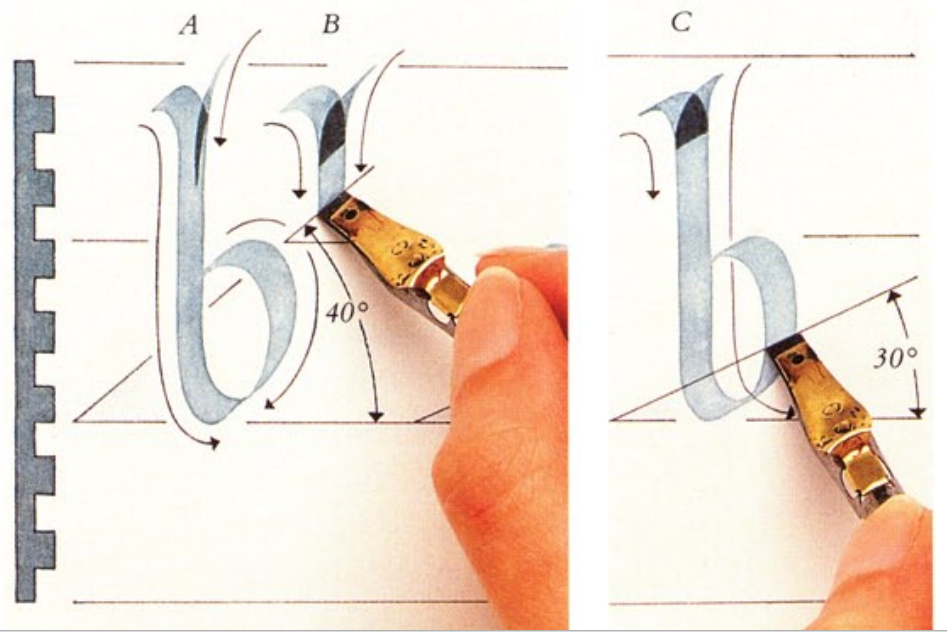
\includegraphics[width=0.75\linewidth]{gliph.png}
\end{frame}
\begin{frame}{Расположение глифов относительно друг друга}
Апрош — расстояние между шрифтовыми знаками.
\begin{itemize}
\item в большинстве СП используется нулевой апрош\\
{\JAP カーニングには多少のデメリットもある。}
\item в моноширинных шрифтах используется нулевой апрош\\
{\small \MON Эй жлоб! Где туз? Прячь юных съёмщиц в шкаф.}
\item в остальных типах шрифтов и некоторых СП используется как отрицательный, так и положительный апрош\\
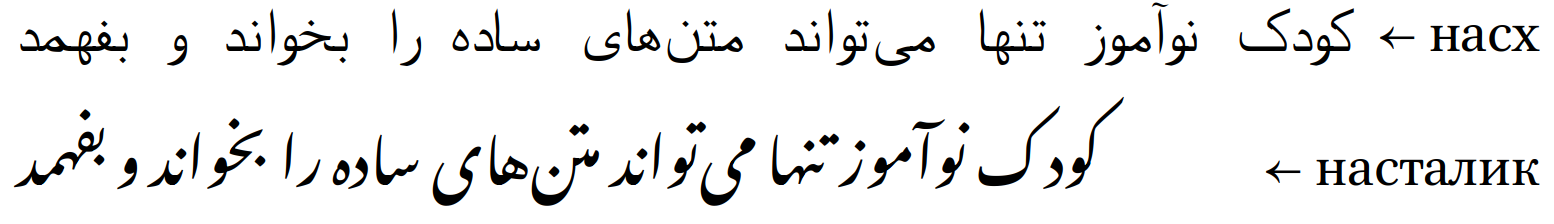
\includegraphics[width=\linewidth]{arabic.png}
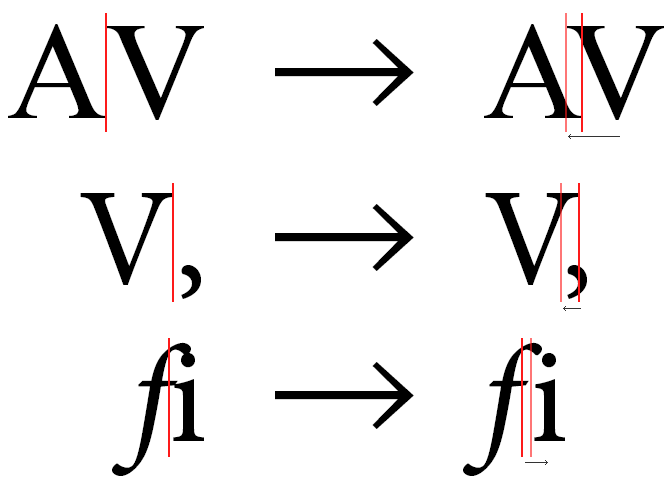
\includegraphics[width=0.4\linewidth]{approche.png}
\hfill ← кернинговые пары
\end{itemize}
\end{frame}
\section{развитие СП}
\begin{frame}[c]{Что влияет на систему письма?}
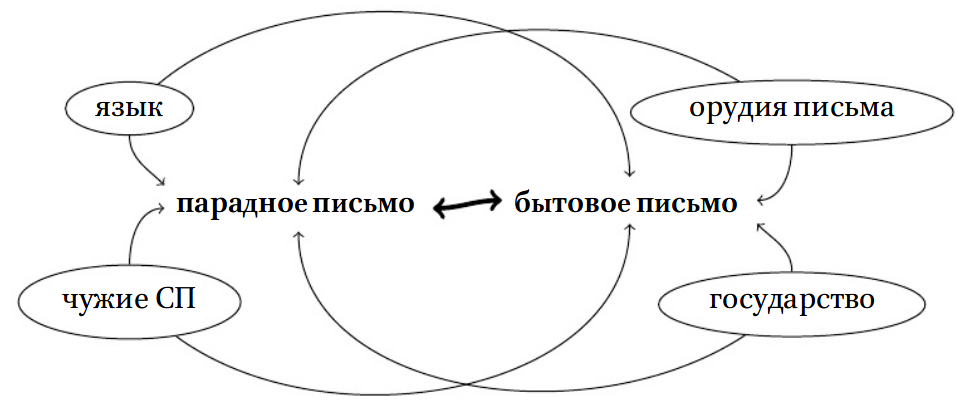
\includegraphics[width=\linewidth]{change.png}
\end{frame}
\begin{frame}{Как развивались системы письма?}
\href{https://player.ooyala.com/iframe.html?ec=lzdjhreTqWkFgF7-l5ECMYfS96wW-R6M&pbid=6e12e8b3387a44daacfb73afba25a76e&options[autoplay]=true}{видео Kuzoian A. (2015) The spread of the world's first writing systems}
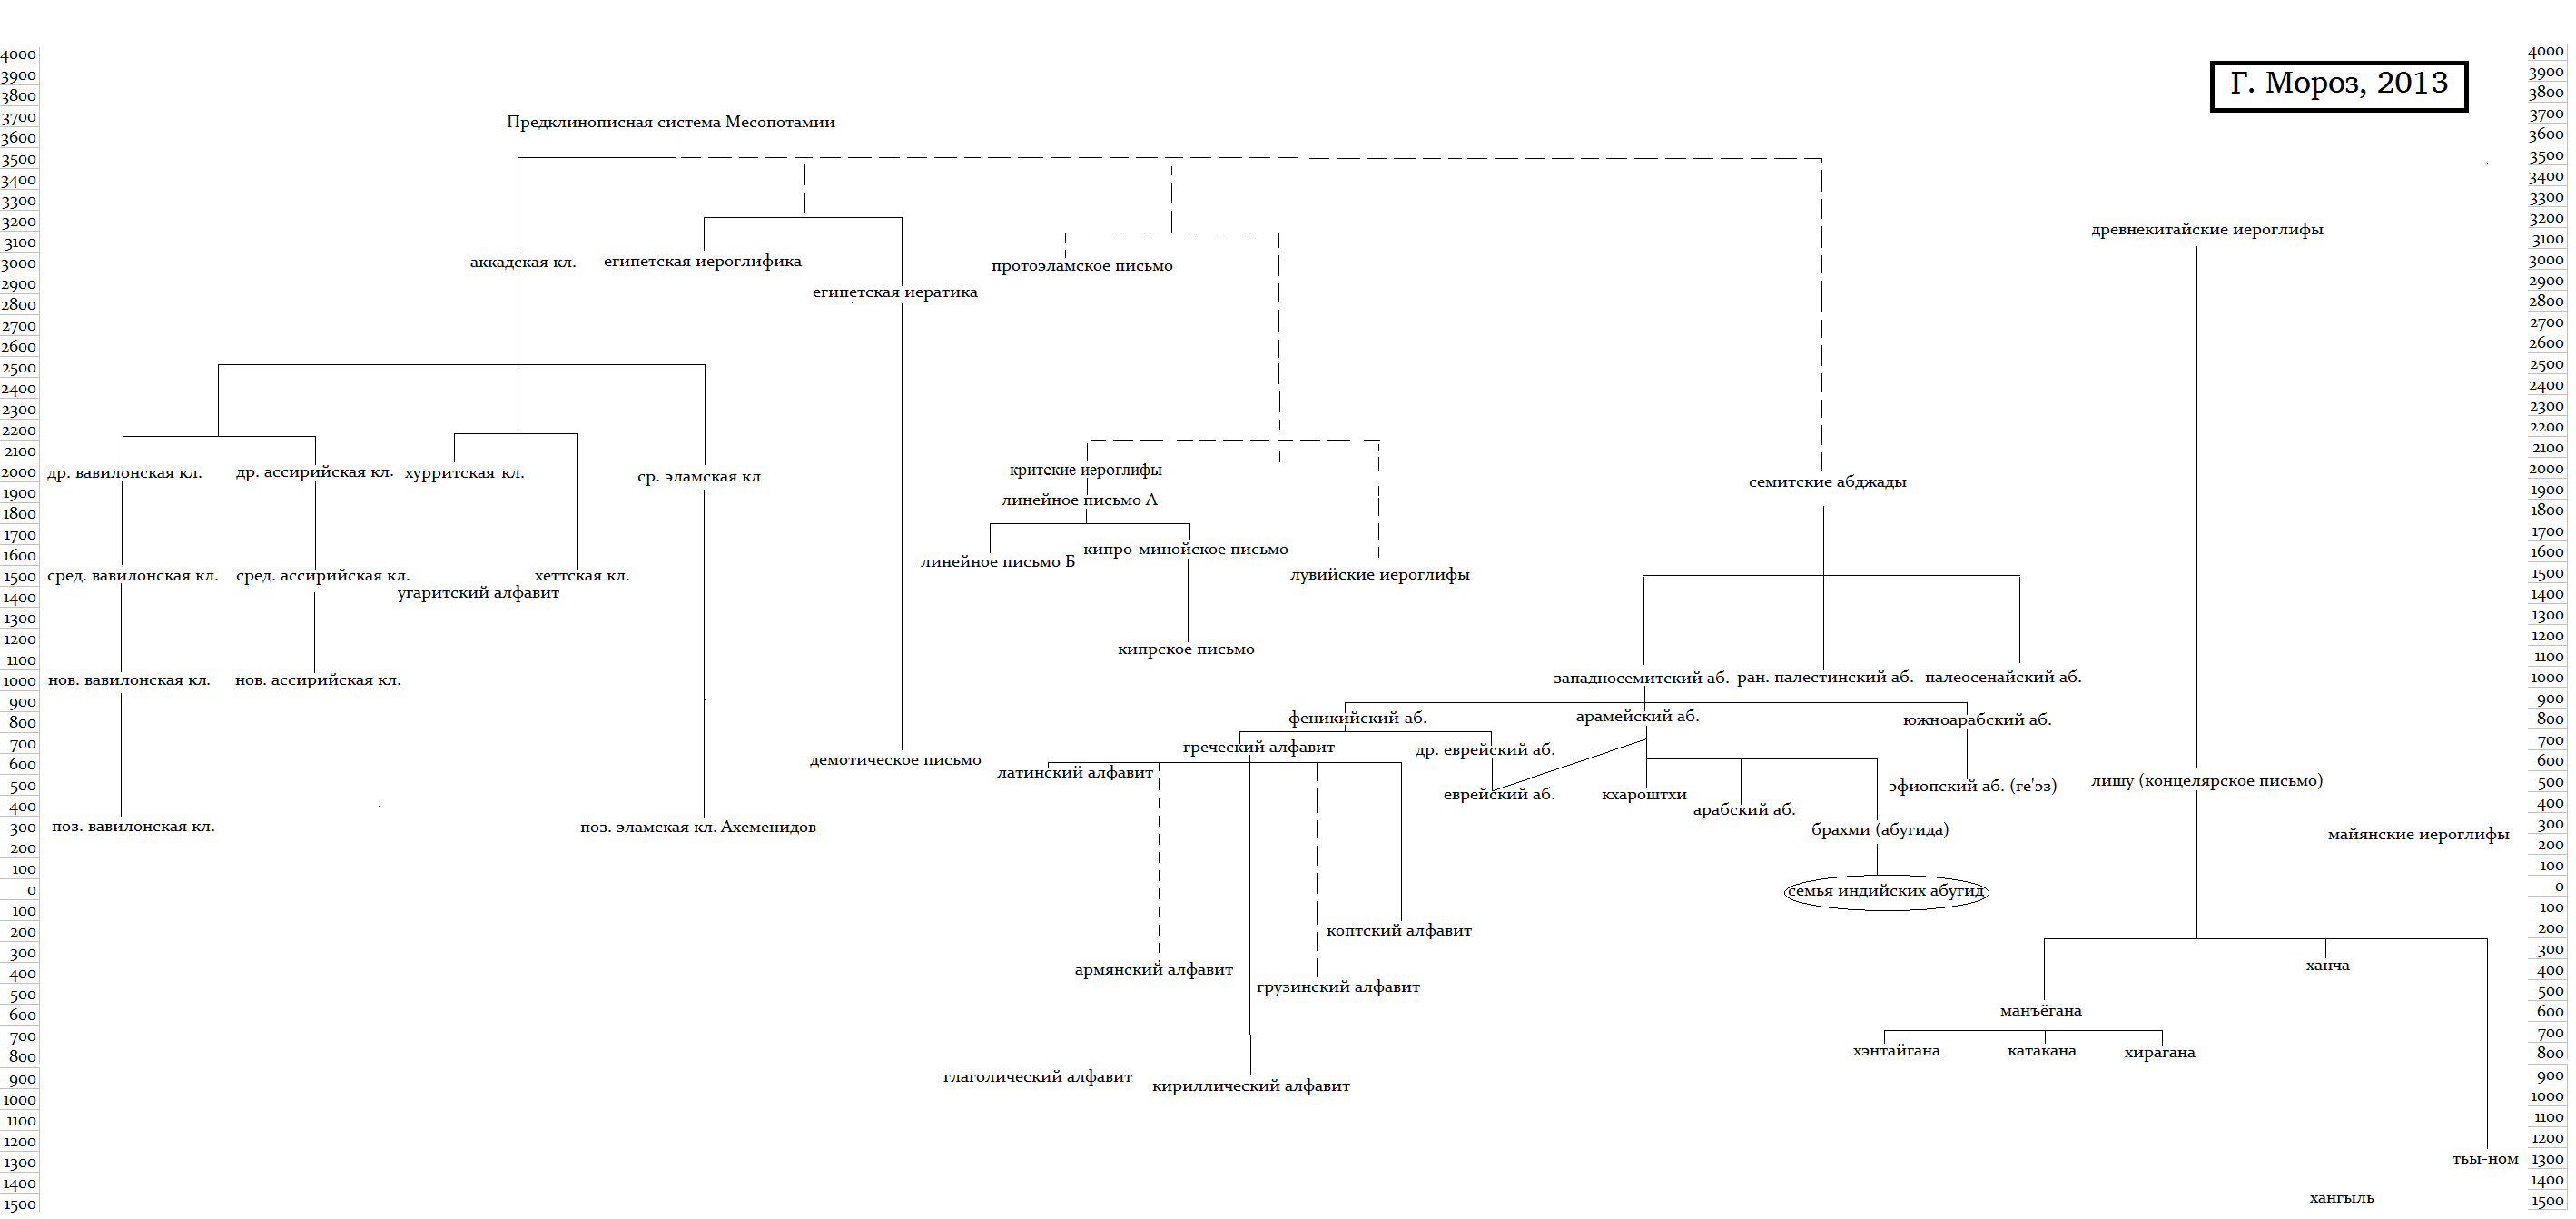
\includegraphics[width=\linewidth]{genealogy.png}
\end{frame}
\section{компоненты СП}
\begin{frame}{Как связаны единицы языка и письма?}
Получившие бурное развитие исследования устного дискурса в 80-ые года достаточно быстро показали, что:
\begin{itemize}
\item лингвисты часто моделируют язык, основываясь на письменном языке
\item письменный и устный языки манипулируют разными единицами (\citep{wackernagel71}, \citep{foster00})
 \end{itemize}
Развитие телевидения и мессенджеров показало, что:
\begin{itemize}
\item письменный текст может быть озвучен
\item устный текст может быть записан
\end{itemize}
\end{frame}
\begin{frame}{Эрратив (eye dialect)}
28 марта 2005 года Роман Лейбов пишет в своем журнале пост под названием ``Тонкости ортографии'':\\
«Беседую с дочкой, сидящей в соседней комнате, по миранде. Спрашиваю, почему она пишет латиницей. Отвечает, что кириллицей надо писать грамотно, а латиницей можно писать \textit{"ne otkrivaecca"}.\\
\textbf{sutasu 06:07 pm:} Многие уже давно перешагнули барьер и спокойно пишут \textit{"не открываецца"}… :-)\\
\textbf{r\_l 06:10 pm:} Я ей то же самое сказал. Но она настаивает, что это — западло.\\
\textbf{sutasu 06:24 pm:} Само наличие понимания, что а) кириллицей надо писать правильно, б) \textit{"не открываецца"} —  это не есть правильный вариант написания, уже достойно восхищения».\\
\hfill из \href{http://www.speakrus.ru/gg/microprosa_erratica-1.htm}{статьи Г. Ч. Гусейнова, 2005}
\end{frame}
\begin{frame}{Эрратив (eye dialect)}
— фонетическая запись слов, не имеющая целью показать неправильное произношение, например, «wimmin» вместо «women», «jamè» вместо «jamais» или олбанский йезыг.
\end{frame}
\begin{frame}{Компоненты системы письма}
\begin{itemize}
\item наборы знаков
\item микроправила соединения знаков\\
\textit{жы-шы}, лигатуры, диграфы, словарные слова
\item макроправила соединения знаков
\begin{itemize}
\item направление письма
\item употребление прописных букв
\item употребление пунктуационных знаков
\item правила переносов
\end{itemize}
\end{itemize}
\end{frame}
\begin{frame}
{\huge Спасибо за внимание!\bigskip\\
\normalsize Пишите письма\\
agricolamz@gmail.com
\vspace{-130pt}}
\end{frame}
%\begin{frame}[allowframebreaks]{Список литературы}
\begin{frame}{Список литературы}
\footnotesize
\bibliographystyle{chicago}
\bibliography{/home/agricolamz/work/bibliography.bib}
\end{frame}
\end{document}